
\documentclass[12pt]{article}

\usepackage{sbc-template}
\usepackage{graphicx,url}
\usepackage{array}
\usepackage{color}
\usepackage{listings}
\usepackage{fancyhdr}
\usepackage[T1]{fontenc}
\usepackage{epsfig}
\usepackage{rotating}
\usepackage{setspace}

\usepackage[square,
            authoryear,
            sort&compress,]{natbib}
\let\cite=\citep

%\usepackage[brazilian]{babel}
\usepackage[latin9]{inputenc}

     
\sloppy
\newcommand{\papertitle}{KnowDIME: An Infrastructure based on Architecture-Driven Modernization for Improving Legacy System}
\title{\papertitle}

\author{Rafael S. Durelli\inst{1,3}, M\'{a}rcio E. Delamaro\inst{1} and Valter V. de Camargo\inst{2}}

 
\address{Computer  Systems Department University of S\~{a}o Paulo\\
  S\~{a}o Carlos, SP, Brazil.
\nextinstitute
  Computing Departament\\ Federal University of S\~{a}o Carlos (UFSCAR)\\
  S\~{a}o Carlos, SP, Brazil.
\nextinstitute
  RMoD Team, INRIA, Lille, France
  \email{\{rdurelli, delamaro\}@icmc.usp.br\inst{1}, valter@dc.ufscar.br\inst{2}}
}

\begin{document} 

\maketitle

\begin{abstract}
%Company runs systems that have been implemented a long time ago. These systems usually are still under adaptation and maintenance to address current needs. Very often, adapting legacy software systems to new requirements needs to make use of new technological advances. 
Legacy systems mainly consist of two kinds of artifacts: source code and databases. Usually, the maintenance of those artifacts is carried out through refactoring processes in isolated manners and without following any kind of standardization. In order to provide a more effective maintenance of the whole system both artifacts should be analyzed, evolved jointly and standardized way. As is known refactoring is a very useful process for dealing with software aging problem since it can improve maintainability and reusability of these system. Recently, researches have been shifted from the typical refactoring processes to the so-called Architecture-Driven Modernization (ADM), which is an approach that follows the all the principles of Model-Driven Development (MDD). As one of the challenges of Software Engineering focuses on mechanisms to support the automation of software refactoring process in this paper we put forward KnowDIME to assist the modernization of a legacy system based on ADM, which uses the Knowledge Discovery Metamodel (KDM) standard. This infrastructure analyses Structured Query Language (SQL) queries embedded in a legacy source code in order to restructure and re-organize the system by using design patterns, such as Data Access Object (DAO) and Service-Oriented Architecture (SOA). 
\end{abstract}
\section{Introduction\label{sec:introduction}}
 Companies have a vast number of operational legacy systems and these systems are not immune to software aging problems. However, they can not be discarded because they incorporate a lot of embodied knowledge due to years of maintenance and this constitutes a significant corporate asset. Furthermore, these kind of systems mainly consist of two artifacts: source code and databases. Usually, the maintenance of those artifacts is carried out through restructuring processes in isolated manners~\cite{Moser:2006}. Nevertheless, we claim that for a more effective maintenance of the whole system both should be analyzed and evolved jointly. 

Refactoring can be used in order to deal with the maintenance of these systems. Martin Fowler~\cite{refactImpro} defines refactoring as ``A change made to the internal structure of software to make it easier to understand and cheaper to modify without changing its observable behavior''. In the literature there is a lot of studies that make refactoring at the level of source code. Empirical studies of refactoring have shown that it can improve maintainability~\cite{1510132} and reusability~\cite{Moser:2006} of legacy system. Not only does existing work suggest that refactoring is useful, but it also suggests that refactoring is a frequent practice~\cite{Murphy:2011}. Cherubini and colleagues` survey indicates that developers rate the importance of refactoring as equal to or greater than that of understanding code and producing documentation~\cite{Cherubini:2007}.

In a parallel research line, researchers have been shifted from the typical refactoring process to the so-called Architecture-Driven Modernization (ADM)~\cite{Ulrich:2010}. ADM has been proposed by OMG (Object Management Group) with the concept of modernizing legacy systems with a focus on all aspects of the current system architecture and the ability to transform current architectures to target architectures. In addition, ADM advocates conducting reengineering processes following the principles of Model-Driven Development (MDD)~\cite{Ulrich:2010:IST:1841736}, i.e., it treats all the software artifacts involved in the legacy system as models and can establish transformations among them.  Firstly a reverse engineering is performed starting from the source code and a model instance (\textbf{P}lataform \textbf{S}pecific \textbf{M}odel - PSM) is created. Next successive refinements (transformations) are applied to this model up to reach a good abstraction level (PSM) in model called KDM (\textbf{K}nowledge \textbf{D}iscovery \textbf{M}etamodel). Upon this model, several refactorings, optimizations and modifications can be performed in order to solve problems found in the legacy system. Secondly a forward engineering is carried out and the source code of the modernized target system is generated again. According to the OMG the most important artifact provided by ADM is the KDM metamodel, which is a multipurpose standard metamodel that represents all aspects of the existing IT (Information  Technology) architectures. The idea behind the standard KDM is that the community starts to create parsers from different languages to KDM. As a result everything that takes KDM as input can be considered platform and language-independent.

Accordingly, one of the challenges of Software Engineering focuses on specifications, architectures and mechanisms to support the automation of software reengineering process, aiming to reduce time and effort spent in this process. Furthermore, legacy systems, often with high maintenance costs due to scarcity or absence of documentation, may be restructured and ported to ADM, providing greater quality in development and maintenance of these systems. Motivated by these ideas, we put forward an infrastructure based on the metamodel KDM which support legacy system reengineering from databases queries and source code, with the objectives of reducing the time and effort in this process and providing migration of these systems to ADM. More specifically, this infrastructure analyses Structured Query Language (SQL) queries embedded in a legacy source code in order to restructure and re-organize the system by using design patterns, such as Data Access Object (DAO) and Service-Oriented Architecture (SOA).  This paper is organized as followed: Section 2 provides information related to the infrastructure - Section 3 the architecture of the infrastructure is depicted - in Section 4 there are related works and in Section 5 we conclude the paper with some remarks and future directions.

%\section{Motivation\label{sec:motivation}} 
% The motivation is the following: (\textit{i}) there is neither a repository, in which the CFs/CFFs can be stored by domain engineer in order to share it, nor an infrastructure where the CFs can be reused as easy as possible in order to disseminate them; (\textit{ii}) most of the CFs found apply white-box reuse strategies - thus it is important provides a way to assist the instantiation of these CFs using models.     

%(\textit{i}) provide an infrastructure to support the reuse of CFs, (\textit{ii}) allowing application engineers to download CF members to be reused in their applications and (\textit{iii}) allowing application engineers to conduct the reuse of CFs in a model-based fashion.  


%In the literature, it is possible find out a large number of researches related to CFF (COLOCAR REF). In these researches a large number of CFF have been devised (e.g., Security, Persistence, Distribution, etc). Thus, it is important develop an environment in which allows engineers share, manage, and provide full cycle of reuse of these CFF. It is also important supplies a graphical way to allow the engineer examines and reuses the features available in one CFF. For instance, the engineer could reuse piece of code of the CFF just selecting a set of features through a feature model.

%Therefore, this environment would increases the quality of the base applications that are developed in terms of modularity, reuse, maintainability. The efficiency will be achieved through the use of techniques related to reuse of analysis, design and code. The quality of the final applications must also be improved with the reuse, since the artifacts have already been tested and approved.  


%For instance, one engineer has developed a CFF and would like to share it in oder to let another engineer reuse his CFF.  CFF has beed developed and  engineer developed a CFF Moreover, it is also important supplies a graphical way to allow the engineer examines and reuses the features available in one CFF. For instance, the engineer could reuse piece of code of the CFF by selecting a set of features in a feature model. % if them fulfill the base application.  the features available fulfilled the base application the engineer would reuse such features.  %whether the features available in one CFF fulfill the base application requirements. 
%To the best of our knowledge there are neither an approach nor a tool with these functionality. In order to overcome such limitations we have put forward a plug-in, in which is described in the next sections.	 

%However, to the best of our knowledge, there is neither an approach nor a tool that allows share, management and also provides full cycle of reuse of the CFF. Moreover, it is important a tool that supplies a graphical way to allow the engineer examines previously if the features available in one CFF fulfill the application requirements. %Moreover, it is important that there is way to allow the engineer verify whether the variability/features available in the CFF meet the application requirements that must be developed.  

%Afterwards, the features have been examined and chosen by the engineer it is likewise important provides a way to download only the artifacts that have been chosen.    

%Thus, the CFF can be used during a development process easier and can be provided major computer support to facilitate such as task.     

%It is important that there is a way to examine whether the variability / features available in the family of FTs meet the application requirements that must be developed. In order for families of FTs to be properly used during a development process, and a major computer support to facilitate this task.


% which implements complete cycle of reuse of the CFF. 
%\textbf{Using this plug-in the CFF can be reused in a controlled way. Thus, during the reuse to increase the quality of the developed applications. Furthermore, any manipulation in the CFF can be made through the intermediary of models, so we intend to raise the level of abstraction in which the engineer works.}


%Thus, the objective of this paper is describes this plug-in. 

%Embora v�rios autores j� tenham trabalhado com FTs (Couto et al., 2005; Hanenberg et al., 2004; Huang et al., 2004; Shah e Hill, 2004; Constantinides e Elrad, 2001; Pinto et al., 2002; Rashid e Chitchyan, 2003; Soares et al., 2006; Vanhaute et al., 2001; Huang et al., 2004; Mortensen e Ghosh, 2006a; Mortensen e Ghosh, 2006b; Soares, 2004), n�o � encontrado na literatura o projeto de um reposit�rio de FTs e t�cnicas para busca de um determinado FT que atenda aos requisitos de uma aplica��o. � importante que exista uma forma de averiguar se as variabilidades/caracter�sticas dispon�veis na fam�lia de FTs atendem aos requisitos da aplica��o que deve ser desenvolvida. Para que fam�lias de FTs sejam adequadamente usadas durante um processo de desenvolvimento, � importante um apoio computacional que facilite essa tarefa.

\section{NOME DA INSFRA\label{sec:proline}} 
In this section our infrastructure is presented. The theory behind it is based on the horseshoe modernization model, which is depicts in Figure~\ref{fig:horseshoe}. As can be seen, this model consist of three steps, \textbf{Reverse Engineering}, (\textit{ii}) \textbf{Restructuring}, and \textbf{Forward Engineering}. The first step is represented by the left side of the horseshoe, it analyzes the legacy system in order to identify the components of the system and their interrelationships. Usually the reverse engineering step builds one or more representations of the legacy system at a higher level of abstraction (PSM). The second one is represented by the curve of the horseshoe since this steps takes the previous system's representation (PSM) and transforms it into another one (\textbf{P}lataform \textbf{I}ndependent \textbf{M}odel - PIM) at the same abstraction level. Finally, the last step is represented by the right side of the horseshoe because it generates physical implementations (source-code) of the target system at a low abstraction level from the previously restructured representation of the system.

\begin{figure}[!h]
\centering
  % Requires \usepackage{graphicx}%left,bottom, right and top
 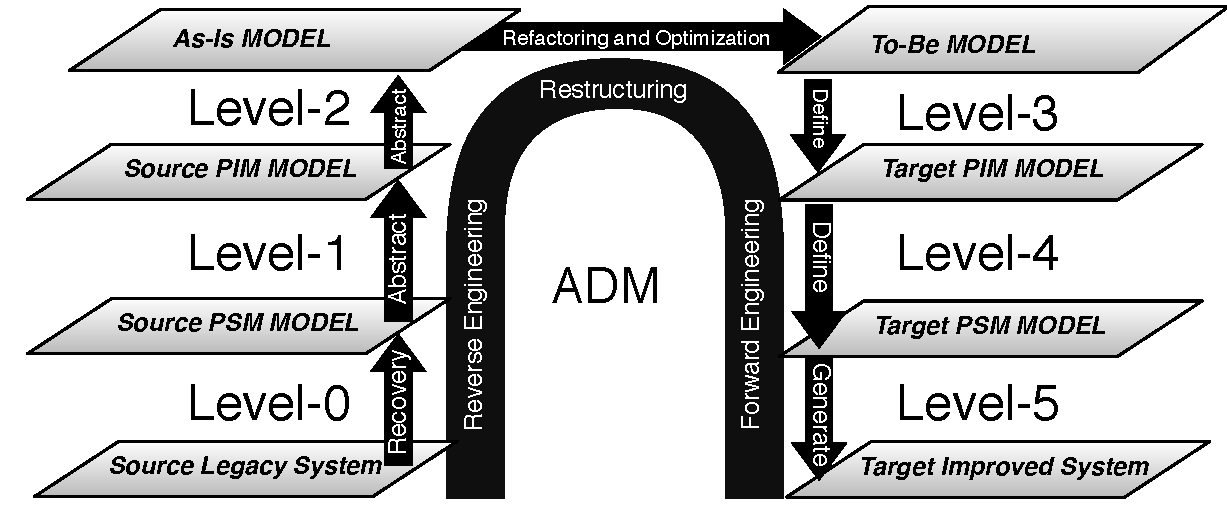
\includegraphics[%scale=0.063, clip=true, trim=32.23cm 18cm 5.45cm 13.853cm
 width=1\textwidth
 ]{Figuras/horseShoeBOM}
\caption{Horseshoe modernization model.}
\label{fig:horseshoe}
\end{figure}

It worth noticing that KDM is the most essential part of our infrastructure. KDM supplies the representation and management of knowledge extracted by means of reverse engineering from all the different software artifacts of the legacy system. Therefore, the legacy knowledge obtained is then modernized into a target improved system by using the concept of MDD. As the infrastructure herein follows the three steps depicts in Figure~\ref{fig:horseshoe} then it has to go through six abstraction levels with five transformations among them. In Figure~\ref{fig:infra} is depicted the infrastructure and also illustrates all abstract levels and the transformations (see the letters `A'- `F'). The Section~\ref{subsection:abstract_level} describes the abstract levels and the Section~\ref{subsection:transformation} explains the transformations.

\subsection{Abstract Levels}\label{subsection:abstract_level}
The \textbf{Level-0} represents all artifacts of the legacy systems in the real world, such as source code and database. The infrastructure uses this artifacts as input to start the ADM process.

The \textbf{Level-1} consist of two PSM. The former model is a source code model, which represents all abstraction of the legacy system's source code, Figure~\ref{fig:infra}(B) illustrates it. More specifically, this model represents an \textbf{A}bstract \textbf{S}yntax \textbf{T}ree (AST), which is a tree representation of the abstract syntactic structure of Java source code. The latter is a database model that illustrates informations related to database used in the legacy system, see Figure~\ref{fig:infra}(A). Similarly, this model is also represented by an AST, the only difference is that it represents syntactic structure of database instead of Java source code. This database model is based on the SQL-92 Data Manipulation Language which can represent the SQL operations such as \textit{Select}, \textit{Delete}, \textit{Update} and \textit{Insert}. %In order to transform the legacy system in these models it is necessary carry out a syntactical analyzer. As for the first model we used a parser that provides a complete self-describing representation of Java source code, i.e., this representation reflects the structure of the software artifact directly in the nesting of elements. Regarding the second model we devised a SQL parser. It consists of a extension of the previously parser but it intends to identify SQL embedded in the legacy system's source code. This parser focus on identifying SQL operations such as \textit{Select}, \textit{Delete}, \textit{Update} and \textit{Insert}; the tables, the columns, primary keys, etc, that appear in these SQL operations are then represented into a AST. Both models, the source code model and the data base model  are represented in the XMI (\textbf{XM}L Metadata \textbf{I}nterchange)-based syntax as can be seen in Figure~\ref{fig:infra} (B) and Figure~\ref{fig:infra} (A), respectively.   


%Both models are deemed as PSM once they owns the software artifact according to their specific technology platforms. 

The \textbf{Level-2} consist of a combination of the two PSMs (see \textbf{Level-1}) for creating a single `As-Is' PIM which is based on the KDM, Figure~\ref{fig:infra}(C) depicts it. This single model makes possible to represent the artifacts of the legacy systems in an integrated and technological-independent way. %The first PSM (source-code) it is transformed to the KDM Code Package, which represents common program elements supported by various programming languages, such as data types, classes, procedures, and templates. In the same way, the second PSM (database model) it is transformed to the KDM Data Package that represents complex data repositories, such as relational databases. 
Afterwards, in the \textbf{Level-3}, by using this PIM the infrastructure allows the software engineer to realize a set of refactoring, refinement and optimizations in such model in order to meet new requirements. %In other words, a set of automated refactoring operations are carried out against the PIM to generate a redesigned PIM. For instance, the software engineer can pick out if he would like to refactor the legacy system to meet either Data Access Object (DAO) or Service-Oriented Architecture (SOA) or both refactorings. As result, new meta-classes may be added to this PIM model, as well as new meta-attributes and meta-relationship in order to meet these requirements. 

Then in \textbf{Level-4} the infrastructure use the PIM redesigned to generate a target PSM, which is represented by a `To-Be' \textbf{U}nified \textbf{M}odeling \textbf{L}anguage - UML model. This model illustrates the target improved system. Finally, in the \textbf{Level-5} the source-code of the target improved system is generated by using the UML as input.

\subsection{Transformation}\label{subsection:transformation}

The first transformation happens between the \textbf{Level-0} to the \textbf{Level-1}. As previously mentioned, this transformation is carried out by following a set of Text-To-Model (T2M) rules in order to obtains two PSM models from legacy system, source code model and database model. To transform the legacy system in these models it is necessary carry out a syntactical analyzer. As for the first model we used a parser that provides a complete self-describing representation of Java source code, i.e., this representation reflects the structure of the software artifact directly in the nesting of elements. Regarding the second model we devised a SQL parser. It consists of a extension of the previously parser but it intends to identify SQL embedded in the legacy system's source code. This parser focus on identifying SQL operations such as \textit{Select}, \textit{Delete}, \textit{Update} and \textit{Insert}; the tables, the columns, primary keys, etc, that appear in these SQL operations are then represented into a AST. Both models, the source code model and the data base model  are represented in the XMI (\textbf{XM}L Metadata \textbf{I}nterchange)-based syntax as can be seen in Figure~\ref{fig:infra} (B) and Figure~\ref{fig:infra} (A), respectively. 

The second transformation is \textbf{Level-1} to \textbf{Level-2}. This transformation is based on a set of Model-To-Model (M2M) patterns to obtain a `As-Is' PIM, which is based on the KDM, see Figure~\ref{fig:infra}. This PIM is generated from the PSM models from \textbf{Level-1}. More specifically, the first PSM (source-code) it is transformed to the KDM Code Package, which represents common program elements supported by various programming languages, such as data types, classes, procedures, and templates. The second PSM (database model) it is transformed to the KDM Data Package that represents complex data repositories, such as relational databases.  

The third transformation \textbf{Level-2} to \textbf{Level-3} realizes a set of M2M operations to transform the `As-Is' PIM to a `To-Be' PIM, i.e., model refactorings and model optimizations are realized in the PIM from \textbf{Level-2}. Therefore, a set of automated model refactorings are carried out against the PIM to generate a redesigned PIM. For instance, the software engineer can pick out if he would like to refactor the legacy system to meet either Data Access Object (DAO) or Service-Oriented Architecture (SOA) or both refactorings. As result, new meta-classes may be added to this PIM model, as well as new meta-attributes and meta-relationship in order to meet these requirements. 

The fourth transformation \textbf{Level-3} to \textbf{Level-4} executes a M2M transformation taking as input the PIM and producing as output a model conforming to the KDM models into UML meta model. The last transformation \textbf{Level-4} to \textbf{Level-5} realizes a set of Model-To-Code (M2C) code generation based on design patterns, such as Data Access Object (DAO) or Service-Oriented Architecture (SOA). The generated code can be complemented by the software engineer in accordance with the more detailed specifications of the application business rules, such as the implementation of specific behaviors and features not covered by the code generation.




\begin{figure}[!h]
\centering
  % Requires \usepackage{graphicx}%left,bottom, right and top
 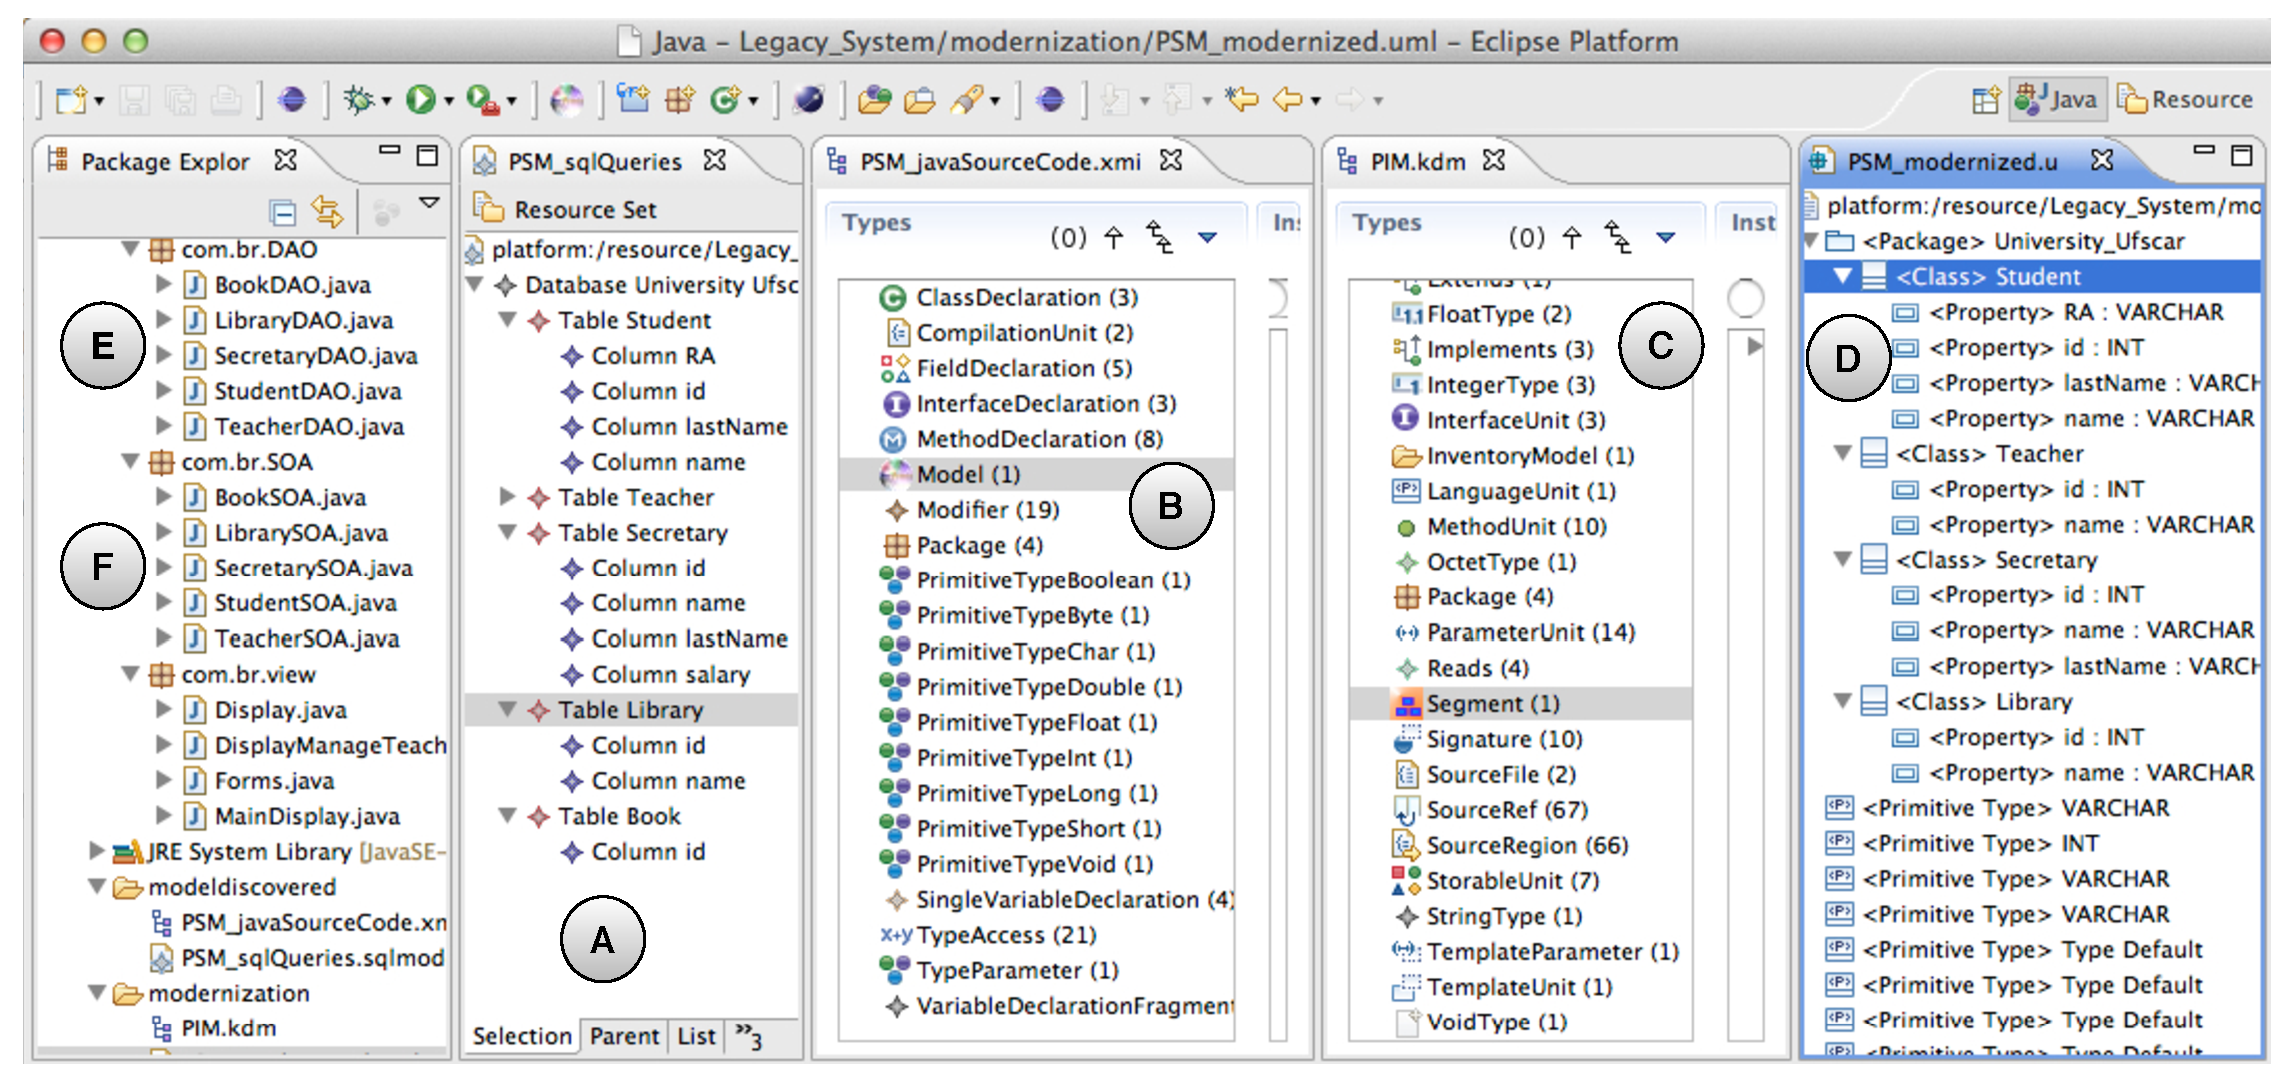
\includegraphics[%scale=0.063, clip=true, trim=32.23cm 18cm 5.45cm 13.853cm
 width=1\textwidth
 ]{Figuras/Tool}
\caption{Screenshot of the Infrastructure}
\label{fig:infra}
\end{figure}

%\subsection{Domain Engineering\label{sec:de}}  
%	%Figure~\ref{fig:proline} depicts a screenshot of ProLine-RM. 
%The DE phase is exhibited by letter ``A'' to ``C'' in Figure~\ref{fig:proline}. 
%In order to illustrated the useful of the ProLine-RM and its functionalities we describe all activities necessaries to devise a ``persistence'' CFF. 
As in development of any framework, firstly the expertise of the domain has to be got.
Therefore, the domain related to ``persistence'' has been studied. 
The outcome of such study were the identification of both the common features and its variants of the domain. 

%After identifying the all features of the CFF the next activity is the development of the CFF. 
In this activity all source code are developed and organized in packages. Each package contain source code (e.g., classes, aspects and methods) related to a feature. %For the purpose of accomplishing this activity we have used the approach described by~\citet{deCamargo:2008:PDC:1363686.1363863}, its aims is to assists and makes easier the develop of the CFF by using aspect oriented paradigm~\cite{Kiczales97aspect-orientedprogramming}. 

Afterwards, the feature model depicting all features related to the domain has to be modeled. 
Aiming to make easier the development of feature models, ProLine-RM provides a graphical way to assists the engineer devises them. 
Figure~\ref{fig:proline}(C) shows the feature model that we have developed. 
As can be seen, there are two set of mandatory features and two groups related to optional features as well.  
%The first one, called ``Persistence'' aims to introduce a set of persistence operations into application persistence classes (e.g., store, remove, update, perform queries). 
%The second feature, named ``Connection'' is related to the database connection concern and identifies points in the application code where the connection must be opened and closed. 
%This feature has variabilities, as for example Data Base Management System (e.g., MySQL, SyBase, Native and Interbase).
%There are two optional features as well. The former is called ``Caching'', which is responsible to deals with high-performance to gets datas of the databases.
%The second, named ``Pooling'' is represented a set of database connections maintained by the databases.

After developing the CFF and the its feature model, them have to be uploaded in a remote repository in order to be reused during the AE phase.
Prior to uploading these artifacts, informations (e.g., Named of CFF, Author(s) and Description) associated with the ``persistence'' CFF has to be filled in. Figure~\ref{fig:proline}(A) shows an example, which the CFF and its feature model are being uploaded. In the next section is described how to reuse the ``persitence'' CFF.

%\subsection{Application Engineering\label{sec:ae}} 
   %%The AE phase is represented by the numbers 1 to 3 as shown in Figure~\ref{fig:proline}. 
%As stated previously, in the AE is wherein the reuse is started effectively.

Firstly, the engineer has to look in the repository and determine whether there are some CFF(s), which can be reused, to make easier and faster the development of the base application. 
In order to assist this activity, ProLine-RM provides a table, which depicts all CFFs that have been uploaded by the engineers in the DE phase.
Figure~\ref{fig:proline}(B) shows this table. 
As can be seen there are six different CFFs - persistence, security, distribution, concurrency, logging and 	Business, respectively. 
In addition, ProLine-RM also shows descriptions for each of the selected CFFs by clicking on the button ``Description''. 
Using this description the engineer can choose the CFFs. 
Nevertheless, if this description is not enough to help the engineer takes a decision on reusing the CFF, ProLine-RM supplies a way visualizes the feature model related to selected CFF by clicking on the button ``View''. 
As is shown in Figure~\ref{fig:proline}(B) the ``persistence'' CFF is highlighted meaning that it has been chosen. 
Next, the ``Download'' button has to be clicked to transfer the feature model belonging to the CFF chosen from the remote repository to the engineer computer.

Secondly, to reuse the CFF its features must be chosen by the engineer aiming to specify explicitly which features will be used in the application base. This is important because usually the CFFs have a great deal of features that probably will not be used in the application base. To assist this activity ProLine-RM uses a file named ``configuration file''. This file is created based on the feature model downloaded. ProLine-RM reads the feature model and creates a ``tree hierarchy''. By using this ``configuration file'' features can be chosen by the engineer. The ``configuration file'' related to the ``persistence'' CFF is shown in Figure~\ref{fig:proline}(D). Moreover, it is interesting to provide a way to validate if the selected features match a valid combination for the instantiation of a member of the CFF, since, certain combinations of features may not lead to useful variants (e.g., in our example the ``persistence'' CFF only a single database connection may be used). ProLine-RM support this validation automatically. As shown in Figure~\ref{fig:proline}(D) once the engineer has chosen the features (represented by ``+''), the resulting variant and constraints are generated automatically (represented by ``-''). 

Finally, the engineer has to submit this validated ``configuration file'' to the remote repository where all CFFs persist. Using this ``configuration file'' the repository will carry out an algorithm. This algorithm aims to extract two artifacts, the codes (e.g., classes, aspects, and packages) related to the features that was chosen by the engineer and a `Reuse Model' (RM), which it is useful to assist the instantiation of CFF's member. After that, these artifacts are sent by the repository to the ProLine-RM. %As can be seen in Figure~\ref{fig:proline}(3) the repository sent only the packages related to the features selected and specified through the ``configuration file'' i.e., the features Persistence, Connection and MySQL.
The application engineer has to filled in the RM. For instance, the value ``base.Custormer.initial'' is a method of the base application and was inserted by the application engineer in the third line of box ``Connection Opening''. After the application engineer fills in the RM with the information needed by an member of a CFF, it is possible to generate the final reuse code.

     
%To the best of our knowledge, there is no an approach that shares, managements, provides full cycle of reuse of the CFF and even supplies a way to examine previously if the features available in one CFF fulfill the application requirements. In order to overcome these absence we put forward an approach and a tool named Proline-RM acronym for Product Line-Repository Manager, which aims to increase the level of manager and accelerate the instantiation of members belonging to a given CFF. The use of the approach is twofold, the Domain Engineering (DE) where all artifacts are developed and upload to a remote server, and the Application Engineering (AE), where the reuse is done effectively. 

\section{Architecture\label{sec:architecture}}
 
%In this section is shown the architecture of the ProLine-RM as well as an description of its components. 
In Figure~\ref{fig:architecture} is depicted the architecture of our infrastructure. As shown in this figure, we devised it on the top of the Eclipse Platform and used both Java and Groovy as programming language. Moreover, we used Eclipse Modeling Framework (EMF)\footnote{http://www.eclipse.org/modeling/emf/} to create the SQL model and to reutilize the UML model. MoDisco is used by the infrastructure since it provides an
\textbf{A}pplication \textbf{P}rogramming \textbf{I}nterface - (API) to easily access the KDM model. 

\begin{figure}[!h]
\centering
  % Requires \usepackage{graphicx}
 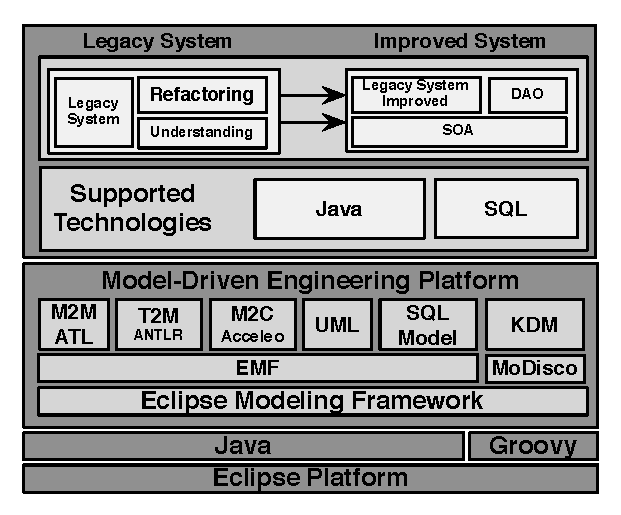
\includegraphics[scale=0.8]{Figuras/Arquitetura_da_Ferramenta}
\caption{Architecture of KnowDIME}
\label{fig:architecture}
\end{figure}



\textbf{A}Nother \textbf{T}ool for \textbf{L}anguage \textbf{R}ecognition -  (ANTLR) is used herein to create parsers to obtain information related to the legacy system's artifacts. Therefore, two parser were developed: (\textit{i}) the first takes as input a Java grammar and generates as output an AST and (\textit{ii}) the second parser is a extension of the first one to identify SQL embedded in the legacy system's source code, i.e., it takes as input a Java source-code and generates as output an AST which contains informations such as, tables, columns, primary keys, etc. Then, to transform these ASTs in PSMs we used an API provided by EMF. Afterwards, all transformation M2M are done by \textbf{A}tlas \textbf{T}ransformation \textbf{L}anguage - ATL, which provides ways to produce a set of target models from a set of source models. Therefore, ATL is used to transform the PSMs to conform the KDM specification and to transform the improved KDM to an UML that represents the target systems. Then, in order to transform this last model in a set of physical artifacts (source code) Acceleo was used, which is based on textual template approach. A template can be thought of as the target text with holes for variable parts. The holes contain metacode which is run at template instantiation time to compute the variable parts. Furthermore, we have used Java Persistence API (JPA) 2.0 to deal with the way relational data is mapped to Java objects. Similarly, RESTful API have been used to implements SOA artifacts.


%Afterwards, all transformation M2M are done by ATL, which is a language...For instance, it is used to transform the PSMs to conform the KDM specification ...into KDM a set of rules were written in ATL, which is a language....., It is used to transform the As-is PIM to a To-be PIM, and finally, to transform this PIM in a PSM conforming the Uml meta model. Then, in order to transform this last model in a set of physical artifacts (source code) Acceleo was used.
 

  %tha  both the source-code of the legacy system and database/SQL queries embedded in into PSM models.


%As can be seen in Figure~\ref{fig:architecture}, all artifacts (source code, feature model, RM and RRM) that the CrossFIRE provides are persisted in a database. These artifacts are persisted in a remote server, available to be reused in the AE phase. This remote server is a physical computer, which is dedicated to run the RESTful API. Therefore, to send these artifacts by the server we have used this API as web service to cache the representation of all artifacts. This server receives requests of the CrossFIRE through RESTful, processes database queries and sends a response to the CrossFIRE by using RESTful as well. Furthermore, we have used Java Persistence API (JPA) 2.0 to deal with the way relational data is mapped to Java objects. To implement the database of the server, the MySQL was chosen.



\section{Related Work\label{sec:related}}
  The approach proposed by Cechticky \textit{et al.}  \citep{Cechticky:2003:GAF:954186.954203} allows object-oriented application framework reuse by using a tool called OBS Instantiation Environment. That tool supports graphical models do define the settings of the expected application to be generated. The model to code transformation generates a new application  that reuses the framework. The proposal found in this paper differs from their approach on the following topics: (\textit{i}) their approach is restricted to frameworks known during the development of the tool; (\textit{ii}) it does not use aspect orientation; (\textit{iii}) the reuse process is applied on application frameworks, %, therefore, %a completely new application is generated.
which are used to create new applications.


 Another approach was proposed by Oliveira \textit{et al.}  \citep{Oliveira:2011:RET:2039458.2039832}. Their approach can be applied to a greater number of object oriented frameworks. After the framework development, the framework developer may use the approach to ease the reuse by writing the cookbook in a formal language known as Reuse Definition Language (RDL) which also can be used to generate the source code.
This process allows to select the variabilities and resources during reuse, as long as the framework engineer specifies the RDL code correctly.

\section{Concluding Remarks\label{sec:conclusion}}
 In this paper is presented the KnowDIME to support the refactoring of legacy systems based on ADM, which uses the KDM standard. It follows the theory of the horseshoe modernization model, which is threefold: (\textit{i}) \textbf{Reverser Engineering}, (\textit{ii}) \textbf{Reestructuring} and  (\textit{iii}) \textbf{Forward Engineering}. 

Firstly, all the artefacts of the legacy system must be transformed into PSMs by statically analyzing the legacy source code. Still in the first step, these PSMs are integrated into a KDM model, i.e., a PIM model, through a M2M transformation implemented using ATL. Secondly, the KnowDIME applies a set of model refactorings and model optimizations in this PIM. Afterwards, KnowDIME executes a set of M2M transformation taking as input the PIM and producing as output a model conforming to the KDM models into UML meta model. Finally, an improved system is obtained from this UML by means of a set of M2C transformation; additionally, the generated code can be complemented by the software engineer in accordance with the more detailed specifications of the application business rules, such as the implementation of specific behaviors and features not covered by the code generation.

We believe that KnowDIME makes a contribution to the challenges of Software Engineering which focuses on mechanisms to support the automation of software refactoring process. Long term future work involves conducting experiments to evaluate the level of maintenance provided by KnowDIME. It is worth highlighting that KnowDIME is open source and it can be downloaded at\textit{~www.dc.ufscar.br/$\sim$valter/crossfire}.


\section{Acknowledgements}
 The authors would like to thank CNPq for Processes 241028/2012-4 and FAPESP for Process 2012/05168-4.

\bibliographystyle{apalike}
\bibliography{referencias}

\end{document}
